\chapter{User Guide}

The user guide is a tutorial for non-technical users to learn how to use the tool. The tool has been extensively tested on Linux. The tool should run on Windows, however no guarentees are made.

\section{Installation}

The tool has the following dependencies:

\begin{itemize}
	\item Python
	\item NumPy
	\item Matplotlib
	\item Tkinter
	\item Pyomo
	\item An optimiser, either CPLEX or GLPK
\end{itemize}

Please refer to their websites for troubleshooting. Alternaitvely, contact the author for assistance.

%\fbox{
	\begin{verbatim}
		sudo apt-get install python3
		sudo apt install python3-pip
		pip3 install numpy
	\end{verbatim}
%}

\section{Usage}

\begin{figure}[H]
	\centering
	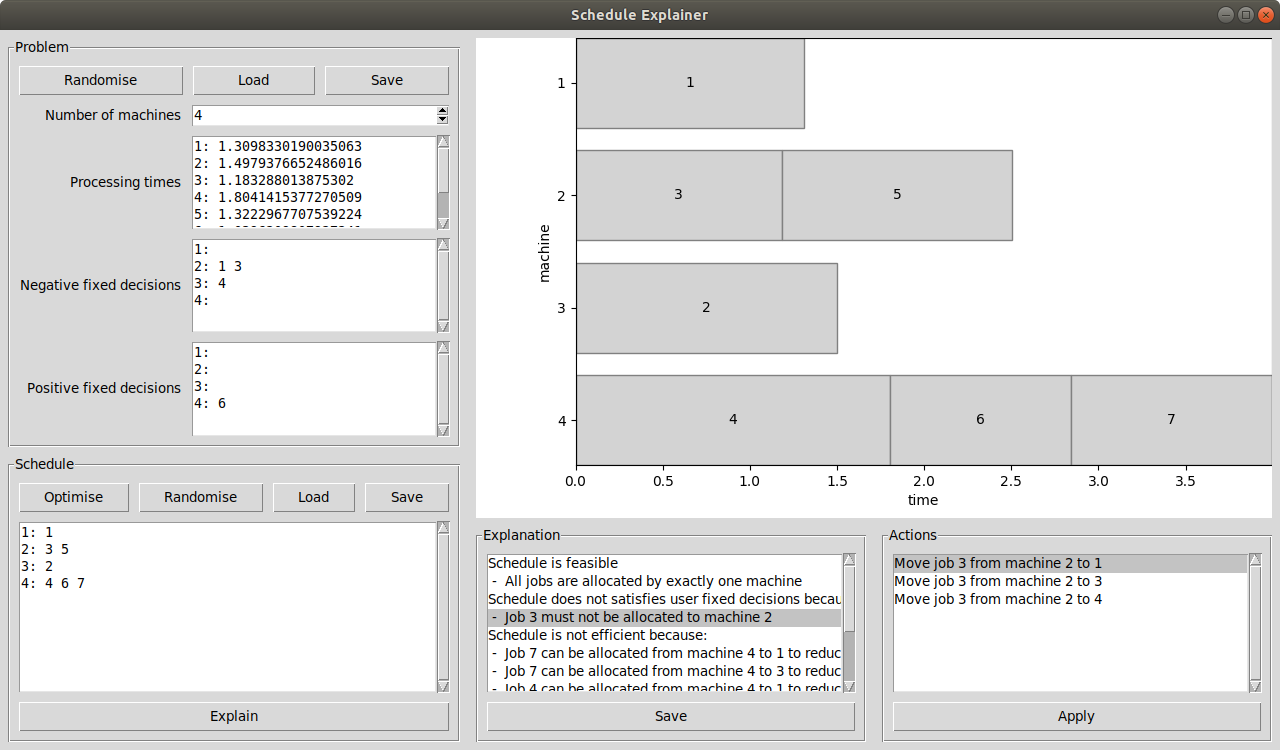
\includegraphics[width=\linewidth]{figures/tool_gui.png}
	\caption{Tool GUI}
\end{figure}



Lorem ipsum dolor sit amet, consectetur adipiscing elit. Fusce volutpat quam eu quam suscipit pharetra. Curabitur mattis nibh id metus feugiat, at blandit velit hendrerit. Quisque venenatis suscipit elit at euismod. Vestibulum ut metus vitae metus luctus tincidunt vitae eu felis. Vivamus eleifend, massa nec dignissim sagittis, eros lectus tempor neque, ac luctus magna purus ac massa. Donec fringilla arcu nec sapien varius, nec convallis justo posuere. Aenean fermentum libero erat, vitae ullamcorper diam commodo non. Nunc sodales accumsan nibh, et pellentesque sapien faucibus sed. Phasellus rhoncus dignissim orci. Aliquam maximus condimentum erat, ut porta augue euismod eu. Vestibulum ac quam ac mauris dignissim euismod vel at turpis. Curabitur nisi mauris, congue sed egestas sed, vulputate eu lorem. Donec sed semper libero. Integer diam lacus, facilisis non risus a, blandit dignissim ex. Nunc mi nulla, condimentum sit amet tellus nec, viverra gravida neque.

\subsection{Startup}

\subsection{Data Input}

\subsection{Explanations}